\documentclass{article}
\usepackage{ifxetex}
\ifxetex
  \usepackage{fontspec}
\else
  \usepackage[T1]{fontenc}
  \usepackage[utf8]{inputenc}
  \usepackage{lmodern}
  \usepackage{float}
  \usepackage{graphicx} 
  \usepackage{morefloats}
  \usepackage{wrapfig}
  \usepackage{babel}
  \usepackage{enumerate}
\fi
  
\begin{document}

\begin{titlepage}
\begin{center}
    \vspace*{-1in}
    \begin{figure}[htb]
    \begin{center}
    
\includegraphics[width=8cm]{escudo-gde-trans.png}
    \end{center}
\end{figure}    
\begin{center}
LICENCIATURA EN FÍSICA \\
\vspace*{0.15in}
DEPARTAMENTO DE FÍSICA \\
\vspace*{0.6in}
\begin{large}
FÍSICA COMPUTACIONAL 1 \\
\end{large}
\vspace*{0.2in}
\rule{80mm}{0.1mm}\\
\vspace*{0.1in}
\begin{large}
\textbf{Evaluación 1\\ }
\end{large}
\vspace*{0.3in}
\begin{large}
Alumna: \\
\vspace*{0.1in}
Brambilla Zamorano Fátima Fernanda\\
\end{large}
\vspace*{0.3in}
\rule{80mm}{0.1mm}\\
\vspace*{0.1in}
\begin{large}
Fecha: \\ 08/03/18\\
\end{large}
\end{center}
\end{center}
\end{titlepage}

\section{Descarga y Depuración de Datos}
En primer lugar descargamos un par de archivos como se nos fue indicado, el primero dada los datos del nivel del mar en el manglar \textit{El Sargento}, y el segundo los de la salinidad en el mismo. Y se nos pido que por medio de los comandos de Linux y Emacs revisaramos que ambos archivos (independientes uno del otro) tuvieran la misma cantidad de lineas, y columnas de datos, así como se nos fue pedido que los editaramos de no ser este el caso. 
De modo que al archivo de los datos de salinidad le borre las últimas dos líneas de datos para que tuviera la misma cantidad de filas que el archivo de los datos del nivel de agua. 

\section{Procedimiento de lectura de Datos}
Lo siguiente fue leer los archivos con Python, por medio del entorno de trabajo de Jupyter Notebook, donde debiamos cargar las bibliotecas que serían requeridas, como "date time", "pandas", entre otras. 
Después de importar las bibliotecas, le indicamos al programa que lea los datos de ambos archivos, y muestra las primeras lineas de la tabla para comprobar que los esta leyendo como es debido.
A continuación, se hizo una transformación de la columna "Date" en los archivos originales, para poder trabajar más comodamente con ella durante el programa que desarrollaría unas gráficas. 
\begin{figure}[htb]
    \begin{center}
    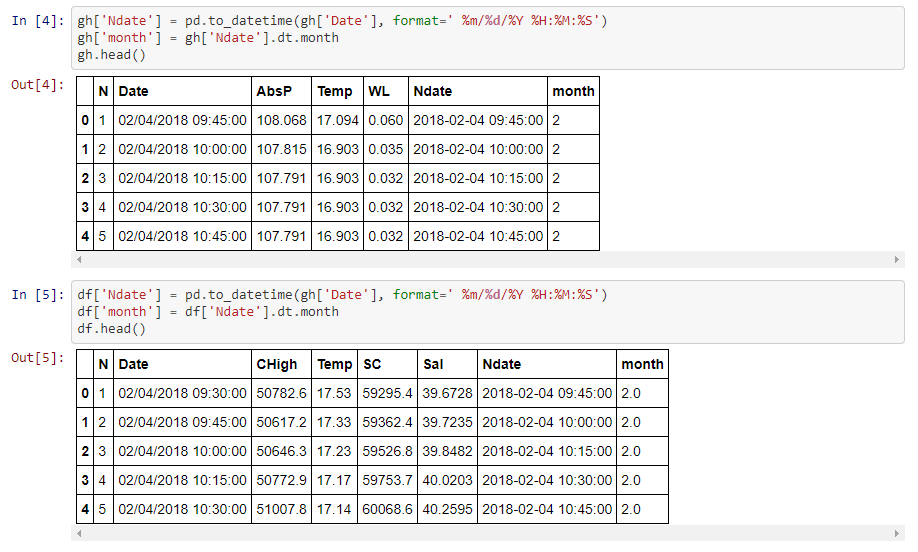
\includegraphics[width=8cm]{CambioDate.PNG}
    \end{center}
\end{figure}  

Una vez editada la columna \textit{Date}, comenzamos a hacer las gráficas correspondientes. En primer lugar, hicimos tres gráficos de caja que mostraban los siguientes datos: 
\begin{enumerate}
\item El nivel del mar
\item La salinidad en partes por millón
\item La temperatura del agua 
\end{enumerate}
Después de hacer las gráficas de caja, utilizamos las función \textit{describe} para calcular los maximos y minimos de los cuartiles.
A continuación, se hicieron gráficas independientes para los mismos datos mencionados anteriormente, esta vez en función del tiempo, de modo que se pudiera ver mejor su comportamiento. En estas últimas gŕaficas pudimos notar como es que estos datos tienen un comportamiento oscilatorio, mostrando varios picos en las gráficas. 
Después de analizar el comportamiento de estas tres variantes, se nos fue pedido que hicieramos gráficas dobles, ver el comportamiento de estas variables en pareja y para ello fue necesario unir los datos de ambos archivos, usando de pormedio una de las funciones de las bibliotecas pandas, concat, para unir las columnas de datos deseados. De este modo fue como si trabajaramos con un tercer archivo de datos, el cual combinaba unicamente las partes deseadas de los archivos leídos previamente. 
Una vez que hicimos este arreglo, fue posible hacer las últimas gráficas requeridas, las cuales tuvieron dos versiones, una con todos los datos del archivo, y la segunda limitando los datos a cinco días de medición, para poder observar mejor el comportamiento que tenian el nivel del agua, la salinidad en esta y su temperatura. 

\section{Gráficas obtenidas}
En esta sección se presentaran las gŕaficas obtenidas a lo largo de la actividad que consistió en la evaluación parcial, así como una breve explicación de cada una de ellas. \\
La primera gráfica corresponde al gráfico de caja de los datos del nivel del agua durante el mes de febrero.
\begin{figure}[htb]
    \begin{center}
    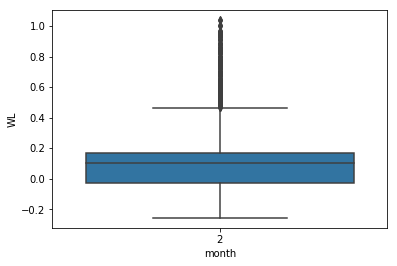
\includegraphics[width=8cm]{BPNivelA.png}
    \end{center}
\end{figure}    
A simple vista no es fácil decir cual es la disperción de datos, sin embargo, es sencillo ver donde se encuentran los cuartiles así como la media de los datos. Para esto, mostrare más adelante una tabla con estos datos mencionados. \\
El siguiente gráfico corresponde al diagrama de caja para los datos de la salinidad del agua durante el mes: \\
\begin{figure}[htb]
    \begin{center}
    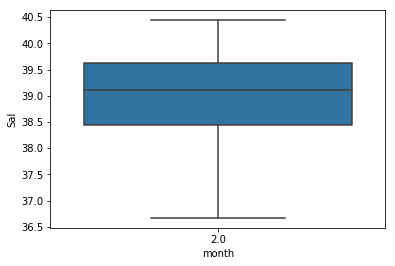
\includegraphics[width=8cm]{BPSalinidad.png}
    \end{center}
\end{figure}    

Al contrario que el caso anterior, la dispersión de datos en la salinidad del agua parece estar menos dispersa, lo cual se puede notar por los puntos que aparecen en la recta en la primera gráfica, fuera de la caja, y que en la segunda gráfica no aparecen. 
Por último, presente el gráfico de caja para los datos de la temperatura. A pesar de que se hizo un gráfico para la temperatura marcada en cada uno de los archivos de datos, ya que estos datos son bastante similares, solo se expondrá una de las gráficas
\begin{figure}[htb]
    \begin{center}
    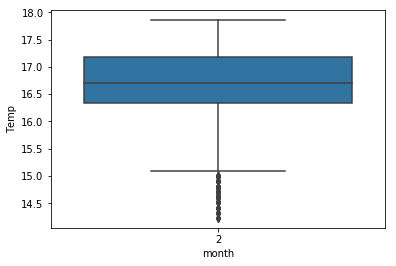
\includegraphics[width=8cm]{BPTemperatura.png}
    \end{center}
\end{figure}    
Como en el caso del gráfico del nivel del agua, se puede observar que hay una dispersión de datos algo grande, ya que algunos de estos salen de la caja y se ven en forma de puntos. 

\begin{figure}[htb]
    \begin{center}
    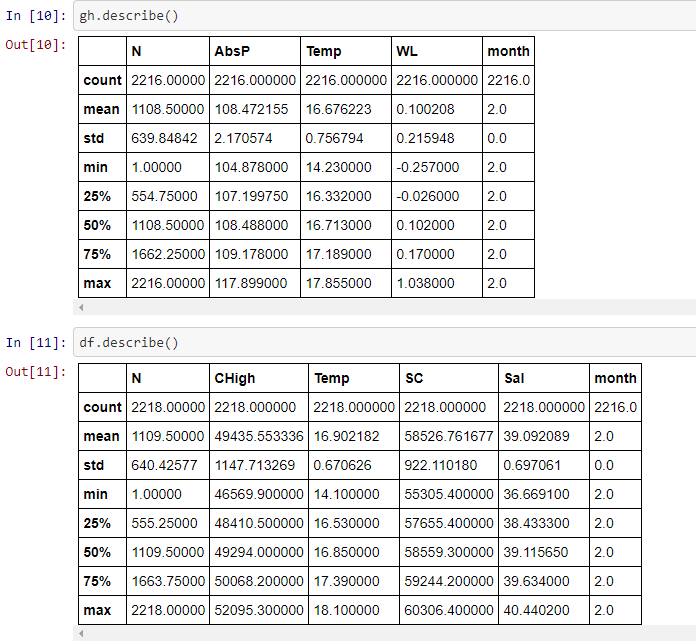
\includegraphics[width=8cm]{Describe.PNG}
    \end{center}
\end{figure}    

En la siguiente imagen se pueden observar los datos que componen las tres gráficas anteriores, siendo la primera tabla correspondiente al archivo de los datos del nivel del agua, y la segunda de los datos de la salinidad de la misma. 

\vspace*{0.5in}

Las siguientes gráficas son las gŕaficas independientes para el nivel del agua, la salinidad en el agua y la temperatura del agua, teniendo las tres variables en función del tiempo. En primer lugar mostraré la del nivel del agua. 

\begin{figure}[htb]
    \begin{center}
    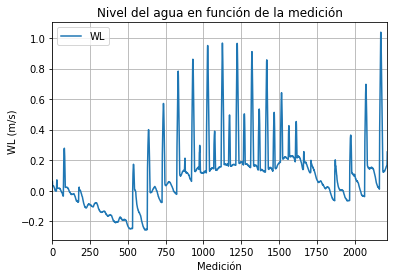
\includegraphics[width=8cm]{AguaMedicion.png}
    \end{center}
\end{figure}    

En esta se puede observar que el comportamiento del nivel del agua es oscilatorio, teniendo altos y bajos a medida que la medición cambia.
La siguiente gráfica es de la salinidad en el agua en función de la medición de datos: 

\begin{figure}[htb]
    \begin{center}
    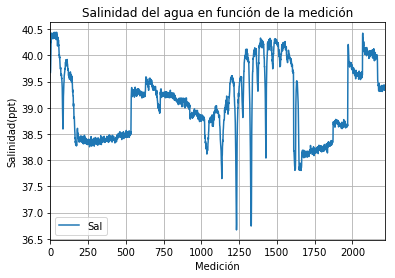
\includegraphics[width=8cm]{SalinidadMedicion.png}
    \end{center}
\end{figure}    

Esta gráfica tiene un comportamiento más extraño si se compará con la gráfica del nivel del agua, no obstante, podría decirse que por tiempos tiene un comportamiento oscilatorio también, solo que sus minimos son más grandes en magnitud que los minimos de los datos en gráfica del nivel del mar. \\
Por último, la gráfica de la temperatura del agua en función de las mediciones hechas 

\begin{figure}[htb]
    \begin{center}
    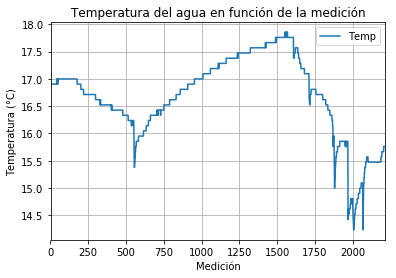
\includegraphics[width=8cm]{TemperaturaMedicion.png}
    \end{center}
\end{figure}  
Esta gráfica tiene un comportamiento bastante diferente a las dos anteriores, por ún lado pareciera que es más estable en cuanto a sus cambios, cosa que hace que sea más sencillo apreciar los cambios en la temperatura a lo largo de cada medición realizada. 

Para continuar la actividad, fue necesario hacer una combinación de los \textit{DataFrames} que teniamos por cada archivo, de manera que tuvieramos un tercer DataFrame que nos combinará únicamente las columnas deseadas, para lo cual se útilizo el siguiente código: 

\begin{figure}[htb]
    \begin{center}
    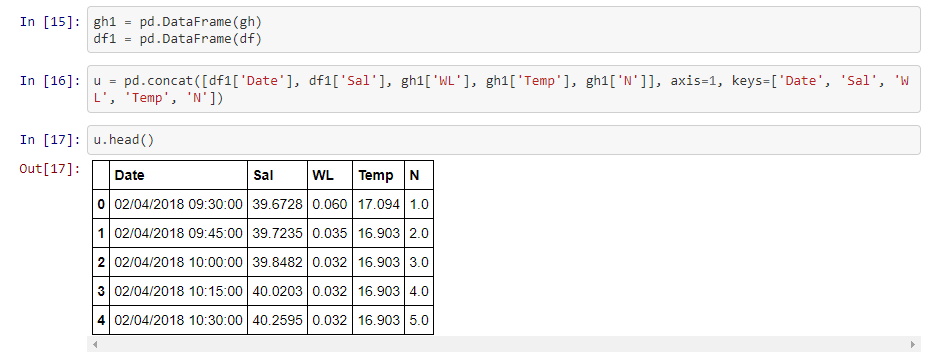
\includegraphics[width=8cm]{MergeData.PNG}
    \end{center}
\end{figure}  

Como se puede apreciar en la imagen, se utilizarón únicamente las columnas que eran compartidas por ambos archivos, como lo era la columna N, la cual era el número de la medición realizada, y la columna Date, que contenía día y hora de la medición, además de unir las dos columnas deseadas, WL que corresponde al nivel del agua, Temp, que corresponde a la temperatura del agua y Sal que corresponde a la salinidad. 
Se hizo esto para poder hacer dos nuevas gráficas, que nos mostrarian en una sola imagen:
\begin{itemize}
\item Nivel del agua y Salinidad
\begin{figure}[htb]
    \begin{center}
    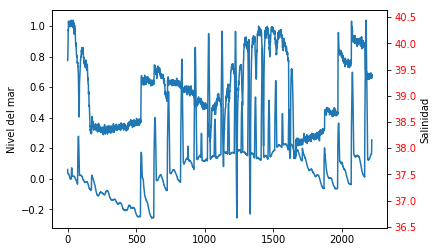
\includegraphics[width=8cm]{NivelAgua-Sal.png}
    \end{center}
\end{figure} 

\vspace{2.5in}
\item Nivel del agua y Temperatura 
\begin{figure}[htb]
    \begin{center}
    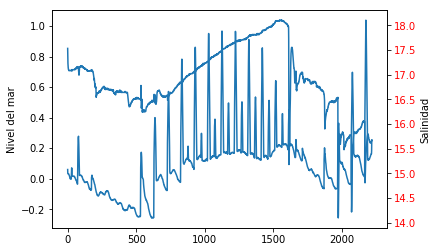
\includegraphics[width=8cm]{AguaTemp.png}
    \end{center}
\end{figure} 
\end{itemize}

Estando ambos casos en función del número de mediciones realizado. Estas gráficas, por falta de tiempo tienen ambas variables del mismo color, por lo que no es sencillo ver cual linea corresponde a cual variable, más adelante tanto este comentario como las gráficas serán editadas. \\

Las últimas gráficas son de nueva cuenta las gráficas independientes del nivel del agua, la salinidad en el agua y la temperatura del agua como funciones del tiempo, esta vez siendo limitadas por las mediciones hechas en cinco días, lo que es se cumple aproximadamente en la medición 285. 
Sin embargo, debido a un error de lectura, no son estas gráficas las que hice, sino que hice dos pares de gráficas que no iban en la actividad, las cuales a pesar que no las mostraré en este documento, pueden verse en \textit{GitHub} 

\end{document}
